\section{Experimental Results}

This section evaluates the self-supervised world models, supervised sequence baselines, and calibrated ensembles across both experimental datasets, followed by feature channel attribution and an edge deployment discussion.

\subsection{Single-Model Classification Performance}

\begin{figure}[!t]
    \centering
    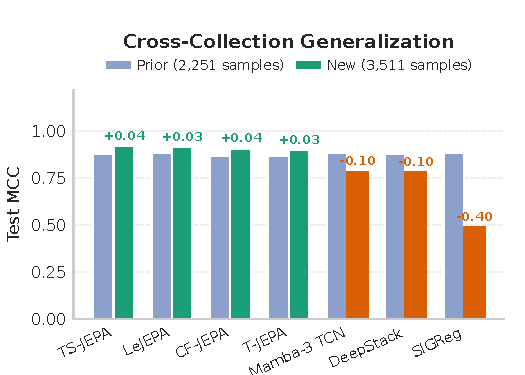
\includegraphics[width=\columnwidth]{images/transfer_mcc.pdf}
    \caption{Cross-collection generalization and single-model test \ac{MCC}. Self-supervised JEPA world models demonstrate positive transfer on the new collection, whereas supervised classifiers and state-space architectures degrade.}
    \label{fig:transfer}
\end{figure}

Models were evaluated across both dataset collections. Table~\ref{tab:single} reports the test \ac{MCC} of each model family on the prior 2,251-sample dataset and on the new 3,511-sample dataset, along with the performance differential $\Delta$. On the new collection, the four self-supervised world models achieve the top results: TS-JEPA reaches an \ac{MCC} of 0.9194, LeJEPA obtains 0.9143, CF-JEPA achieves 0.9083, and T-JEPA attains 0.8982. Every evaluated \ac{JEPA} architecture substantially exceeds the 0.756 classical Gaussian Process baseline \cite{ribeiro2026eucnc}.

By contrast, the selective state-space Mamba-3 TCN architecture scores 0.7816, and the DeepStack hierarchical ensemble reaches 0.7811. The supervised SIGReg classifier drops to 0.4872 despite leading the prior dataset at 0.8858, and the hyperparameter-optimized GRU baseline attains 0.5746. Figure~\ref{fig:transfer} illustrates this cross-collection transfer behavior.

Multi-seed evaluations across three independent runs (seeds 3, 5, 42) confirm protocol stability, with standard deviations constrained within narrow bounds ($\sigma \approx 0.008$ for SIGReg). Full pretraining over 300 to 500 epochs is mandatory: fine-tuning from early checkpoints (below 100 epochs) collapses test \ac{MCC} to 0.49--0.60 across all seeds.

\begin{table}[t]
    \caption{Single-model test \ac{MCC} on prior \cite{matos2026icaisf} and new collections. $\Delta$ denotes the test \ac{MCC} difference.}
    \label{tab:single}
    \centering
    \small
    \begin{tabular}{lccc}
        \toprule
        Model Architecture & Prior  & New    & $\Delta$ \\
        \midrule
        TS-JEPA            & 0.8785 & 0.9194 & +0.041   \\
        LeJEPA             & 0.8850 & 0.9143 & +0.029   \\
        CF-JEPA            & 0.8661 & 0.9083 & +0.042   \\
        T-JEPA             & 0.8694 & 0.8982 & +0.029   \\
        Mamba-3 TCN        & 0.8844 & 0.7816 & $-0.10$  \\
        DeepStack          & 0.8810 & 0.7811 & $-0.10$  \\
        SIGReg             & 0.8858 & 0.4872 & $-0.40$  \\
        HPO GRU            & 0.8524 & 0.5746 & $-0.28$  \\
        \bottomrule
    \end{tabular}
\end{table}

\subsection{Cross-Collection Generalization and Transfer Invariance}

The cross-collection results in Figure~\ref{fig:transfer} and Table~\ref{tab:single} highlight a key finding: while all self-supervised world models exhibit positive transfer from the prior to the new collection (gaining +0.029 to +0.042 in \ac{MCC}), supervised models and state-space architectures degrade.

The collapse of the supervised SIGReg classifier ($-0.40$ in \ac{MCC}) exposes the vulnerability of purely supervised regularizers to environmental radio shifts. In SIGReg, the Empirical Characteristic Function regularizer penalizes deviations from an isotropic Gaussian latent prior conditioned strictly on the class labels of the training split. Under the richer multi-device interference and channel fading of the new collection, this supervised constraint creates brittle decision boundaries tailored to training artifacts. Conversely, self-supervised \ac{JEPA} pretraining optimizes a predictive objective directly over radio sequence dynamics without label guidance, extracting latent motion invariants that generalize robustly across collection environments.

\subsection{Calibrated Ensemble Performance and Pareto Efficiency}

\begin{figure}[!t]
    \centering
    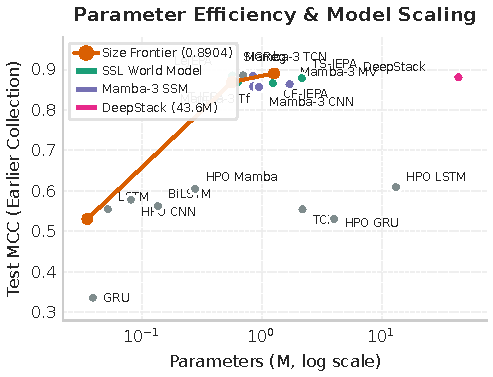
\includegraphics[width=\columnwidth]{images/param_efficiency.pdf}
    \caption{Parameter efficiency frontier. Each point denotes an individual model; the solid curve traces the greedy Pareto selection from logistic regression through LeJEPA to SIGReg.}
    \label{fig:params}
\end{figure}

Table~\ref{tab:ensemble} summarizes ensemble performance and parameter scaling across datasets. Softmax probabilities are temperature-calibrated on validation \ac{NLL} before fusion. On the prior collection, multinomial logistic regression stacking ($C = 0.005$) and entropy-weighted probability averaging both achieve an \ac{MCC} of 0.8873, outperforming uniform probability averaging (0.8814) and Caruana selection (0.8706).

On the primary 3,511-sample collection, the 21-member calibrated logistic regression stack attains a peak test \ac{MCC} of 0.9232, scoring 0.9563 on multi-device noise and 0.9596 on pure single-device traces. The 16-member non-redundant subset matches this peak performance (0.9232 \ac{MCC}) while omitting weak recurrent backbones. For resource-constrained edge execution, the compact 3-member self-supervised subset (\ac{TS-JEPA}, LeJEPA, and \ac{SIGReg}) attains 0.9160 \ac{MCC} with only 3.42~M parameters.

Figure~\ref{fig:params} plots test \ac{MCC} against parameter footprint across four orders of magnitude (0.039~M for GRU to 43.576~M for DeepStack). Self-supervised world models cluster tightly in an optimal high-performance zone between 0.566~M and 2.153~M parameters. While greedy Pareto selection on the prior collection identified a minimal 1.26~M parameter ensemble (logistic regression, LeJEPA, and \ac{SIGReg}) achieving 0.8904 \ac{MCC}, this specific subset drops to 0.5753 on the new collection due to the domain shift collapse of supervised \ac{SIGReg}. In contrast, self-supervised world model ensembles deliver robust transfer across both environments (0.9065 to 0.9160 \ac{MCC}), demonstrating near-peak accuracy at a fraction of the computational footprint.
\begin{table}[t]
    \caption{Ensemble classification performance and parameter scaling.}
    \label{tab:ensemble}
    \centering
    \scriptsize
    \setlength{\tabcolsep}{3.5pt}
    \begin{tabular}{lccccc}
        \toprule
        Ensemble             & $n$ & Params          & Prior           & New             & Noise / Pure                      \\
        \midrule
        21-member full stack & 21  & 74.8~M          & 0.8873          & \textbf{0.9232} & \textbf{0.9563} / \textbf{0.9596} \\
        16-member subset     & 16  & 73.2~M          & 0.8873          & \textbf{0.9232} & \textbf{0.9563} / 0.9179          \\
        World-only stack     & 7   & 6.68~M          & 0.8872          & 0.9065          & 0.9450 / \textbf{0.9596}          \\
        Best-world subset    & 3   & 3.42~M          & 0.8784          & 0.9160          & 0.9341 / 0.8773                   \\
        Three-member Pareto  & 3   & \textbf{1.26~M} & \textbf{0.8904} & 0.5753          & 0.9396 / 0.9179                   \\
        \bottomrule
    \end{tabular}
\end{table}

\subsection{Channel-Level Interpretability and Feature Ablation}

\begin{figure}[!b]
    \centering
    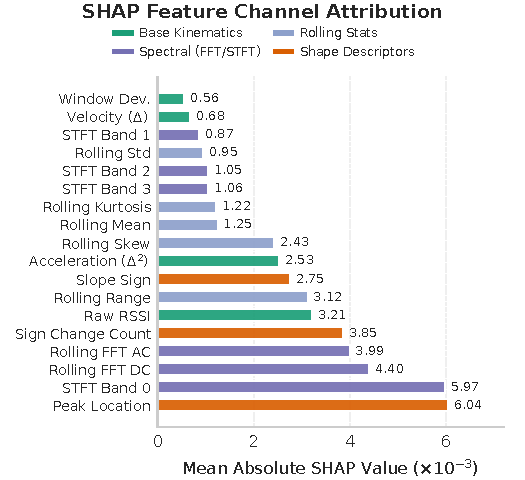
\includegraphics[width=\columnwidth]{images/feature_importance_18ch.pdf}
    \caption{Channel-level \ac{SHAP} feature attribution across the 18-channel hierarchy evaluated on the leading \ac{TS-JEPA} world model.}
    \label{fig:feature_importance}
\end{figure}

To determine how each channel in the 18-channel hierarchy informs latent world-model predictions, we conduct additive feature attribution via \ac{SHAP} on the primary dataset. Figure~\ref{fig:feature_importance} reports the mean absolute Shapley value $|\phi_j|$ per channel evaluated on the leading \ac{TS-JEPA} model.

The attribution hierarchy reveals that macroscopic signal shape and low-frequency spectral power dominate the decision space. Peak location index ($|\phi| = 6.04 \times 10^{-3}$) and low-frequency STFT Band~0 ($5.97 \times 10^{-3}$) contribute most strongly, capturing the exact timestamp of door transitions and the coarse Doppler shifts of physical motion. These are followed by rolling FFT DC power ($4.40 \times 10^{-3}$) and AC energy ($3.99 \times 10^{-3}$), which reflect baseline energy shifts between vehicle zones. In contrast, fine-grained statistical descriptors, such as rolling kurtosis ($1.22 \times 10^{-3}$), rolling standard deviation ($0.95 \times 10^{-3}$), and high-frequency STFT bands, exhibit negligible marginal value, primarily capturing non-semantic multipath scattering rather than transit kinematics.

\begin{table}[t]
    \caption{Architecture-controlled feature channel ablation across world models on the primary dataset (\ac{MCC}).}
    \label{tab:pruning}
    \centering
    \scriptsize
    \setlength{\tabcolsep}{2.5pt}
    \begin{tabular}{lcccc}
        \toprule
        Feature Configuration                            & $C$ & \ac{TS-JEPA}    & CF-JEPA & T-JEPA \\
        \midrule
        Full 18-Channel Hierarchy                        & 18  & \textbf{0.9194} & 0.9083  & 0.8982 \\
        Top-12 \ac{SHAP} Channels                        & 12  & 0.5815          & 0.8098  & 0.5856 \\
        Base Kinematics (Raw, $\Delta$, $\Delta^2$, Dev) & 4   & 0.4486          & 0.4366  & 0.4787 \\
        Rolling Statistics (Moments, Range)              & 5   & 0.3447          & 0.4351  & 0.4944 \\
        Spectral Domain (FFT, STFT 0--3)                 & 6   & 0.2981          & 0.1869  & 0.2283 \\
        Raw \ac{RSSI} Only (Single Channel)              & 1   & 0.2431          & 0.3305  & 0.3395 \\
        \bottomrule
    \end{tabular}
\end{table}

To validate these attribution findings under controlled conditions, Table~\ref{tab:pruning} presents an architecture-controlled feature ablation across \ac{TS-JEPA}, CF-JEPA, and T-JEPA. When input channels are restricted to individual functional domains or the 4-channel base kinematic subset under identical model architectures, performance drops significantly (e.g., from 0.9194 to 0.4486 \ac{MCC} for \ac{TS-JEPA} on 4 channels, and to 0.2431 on raw \ac{RSSI} alone). This confirms that self-supervised world models critically rely on cross-domain synergy across kinematic, spectral, and statistical features to construct noise-invariant latent representations under multi-device interference. At the same time, specialized lightweight architectures designed specifically for low-dimensional inputs, such as LeJEPA (0.566~M parameters, 4 channels), achieve 0.9143 \ac{MCC}, demonstrating that edge access points can choose between rich multi-channel tokenization and ultra-compact dedicated models with virtually zero performance loss.
\subsection{Discussion: Architectural Insights and Sensing Trade-offs}

The experimental findings offer three primary insights into passive ISAC for urban transit using self-supervised world models.
First, the contrast between self-supervised world models and supervised sequence baselines across dataset collections reveals the fundamental mechanism of radio representation learning. In radio sensing, concurrent transmitting devices introduce non-stationary interference that alters local signal distributions. Supervised classifiers regularized with strict isotropic Gaussian priors, such as \ac{SIGReg}, constrain the latent space around training distributions; when unobserved multi-device interference patterns appear, these rigid decision boundaries deteriorate, causing a 0.40 drop in test \ac{MCC}. In contrast, self-supervised \ac{JEPA} pretraining optimizes a predictive objective directly across masked time-frequency patches without label supervision, learning smooth, invariant latent trajectories corresponding to physical passenger displacement.

Second, the channel-level \ac{SHAP} attribution and controlled ablation demonstrate that rich feature synergy is essential for general-purpose world models. Kinematic extrema, low-frequency Doppler power, and baseline energy shifts provide complementary physical constraints. While reducing input dimensions degrades fixed 18-channel patch tokenizers, compact architectures like LeJEPA deliver 0.9143 test \ac{MCC} directly over 4 base channels, confirming flexible edge deployment options.

Third, the Pareto parameter efficiency analysis demonstrates that massive neural ensembles are unnecessary for robust passive sensing. While the 21-member ensemble requires 74.8~M parameters across multiple deep sequence backbones, a compact three-member world model ensemble achieves 0.9160 test \ac{MCC} at only 3.42~M parameters on the primary collection. This confirms that compact self-supervised ensembles deliver state-of-the-art opportunistic sensing with minimal memory footprint, establishing a practical dual-function sensing layer on existing wireless infrastructure.
